% Bridge Actually Received <= Bridge Logged Received
% Bridge Logged Withdraw >= Bridge Actually Withdraw
\begin{figure*}[h]
\centering
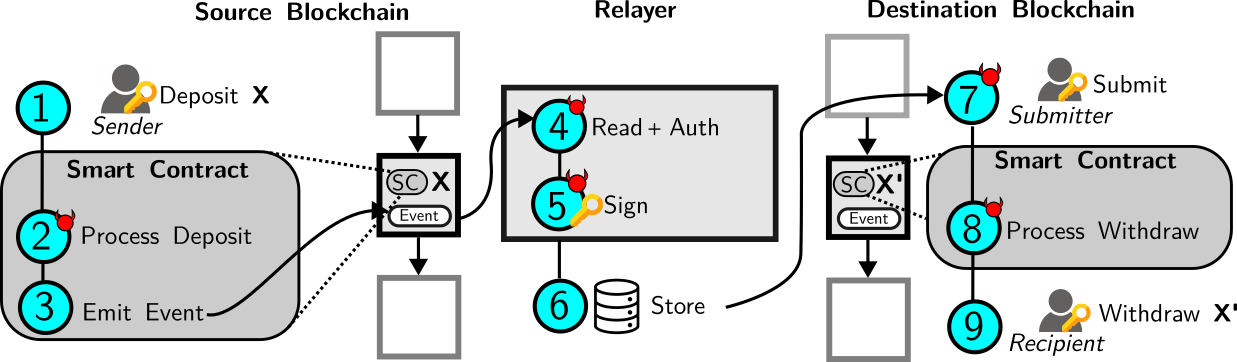
\includegraphics[width=0.8\textwidth]{fig/bridge_arch.pdf}
%%command for cropping pdf
%%gs -sDevice=pdfwrite -o bridge_arch_crop.pdf bridge_arch.pdf
\caption[Cross-chain Token Bridging]{Cross-chain token bridging and the different steps attackers can exploit to withdraw unbacked deposits.}
\label{fig:cross-chain}
\end{figure*}

\section{Background}
\label{sec:background}
% In this section, I start by providing an overview of blockchain technology. We then describe how cross-chain bridges work followed by the threat model I consider in this paper.
% In this section
I first give a brief introduction to smart contract blockchains
and cross-chain bridges. I then describe how bridges, under attack, collapse in
practice.

\subsection{Smart-contract Blockchains} Modern DeFi protocols (e.g.,
decentralized exchanges and lending protocols) are built on top
of ``smart-contract'' blockchains, like Ethereum. At their core, these chains, like
the original Bitcoin blockchain, are distributed ledgers that manage accounts
(public keys) and their balances (in native tokens like Ethereum's ETH). Users
interact with these chains by signing and broadcasting (to the distributed nodes
that make up the chain network) transactions that, for example, transfer
funds from their account (using the corresponding account private key) to
another user's account.

Ethereum, and the smart-contract chains it inspired since its release in 2015,
differ from Bitcoin by extending the ``simple'' distributed ledger with a smart
contract execution layer. A smart contract on Ethereum is an \emph{internal}
account---and, like a normal, \emph{externally owned} account (EOA), it has a
balance---that has associated \emph{code} (EVM bytecode), which implements the
smart contract's program logic, and \emph{storage}, which persists the program's
state across executions. Users interact with (i.e., execute) smart contracts
much like they do when transferring funds from their account: they sign a
transaction that encodes the smart contract to call (i.e., the contract address),
the particular function to execute, and the arguments to call the function with.
Instead of simply transferring funds from the user's account, then, executing
such a \emph{smart-contract call} transaction amounts to executing the smart
contract bytecode---and any smart contracts the contract itself calls.
    
% \begin{lstlisting}
% contract USDC{
%   mapping(account => amount) _balances;
%   event Transfer(from, to, value);
%   function transfer(to, amount) {
%     address from = msg.sender; // user
%     // ... validate user has enough balance
%     _balances[from] -= amount;
%     _balances[to] += amount;
%     emit Transfer(from, to, amount);
%   }

%   function mint(to, amount) {
%     _balances[to] += value;
%     emit Transfer(address(0), to, amount);
%   }

%   function burn(from, amount) {
%     // ... validate user has enough balance
%     _balances[from] -= amount;
%     emit Transfer(from, address(0), amount);
%   }

%   function safeTransferFrom(from, to, amount){ 
%     // ... transfer tokens; revert if failed
%   }
% }
% \end{lstlisting}


\begin{figure}[t]
    \centering
    \includegraphics[width=0.7\columnwidth]{fig/usdc-contract-2sp.pdf}
    \caption{Simplified USDC ERC-20 Token Contract.}
    \label{fig:erc20}
\end{figure}


    

% \lstdefinestyle{myStyle}{
%     belowcaptionskip=1\baselineskip,
%     breaklines=true,
%     % frame=none,
%     % numbers=none, 
%     basicstyle=\footnotesize\ttfamily,
%     % keywordstyle=\bfseries\color{green!40!black},
%     % commentstyle=\itshape\color{purple!40!black},
%     % identifierstyle=\color{blue},
%     backgroundcolor=\color{gray!10!white},
%     language=Python,
% }

% \lstdefinestyle{customc}{
%   belowcaptionskip=1\baselineskip,
%   breaklines=true,
%   frame=L,
%   xleftmargin=\parindent,
%   language=Python,
%   showstringspaces=false,
%   basicstyle=\footnotesize\ttfamily,
%   keywordstyle=\bfseries\color{green!40!black},
%   commentstyle=\itshape\color{purple!40!black},
%   identifierstyle=\color{blue},
%   stringstyle=\color{orange},
% }


\subsection{ERC-20 Tokens}
One of the immediate applications of smart contracts---and to date still one of
most popular---is to create custom tokens (or coins).  To launch a new token, an
organization no longer needs to launch a new blockchain; they can instead deploy
a new contract that implements the ERC-20 token standard interface on a chain
like Ethereum and take advantage of existing on-chain infrastructure like
decentralized exchanges that make it easy to, for example, trade one kind of
token for another---both native tokens (e.g., ETH) and other tokens.\footnote{
    Most EVM chains, i.e., chains that use Ethereum's execution layer,
    follow Ethereum standards like ERC-20. Most non-EVM chains like Solana
    (which have different execution models) have similar standards (e.g., SPL
    tokens in Solana's case).
}

Figure~\ref{fig:erc20} shows a simplified variant of one such token
contract---the USDC \emph{stablecoin} contract.  This contract tracks
how many USDC tokens an account has and governs the spending of these
tokens (much like a bank governs bank notes).  For example, the
contract's \texttt{mint} function lets Circle (the company that owns
the USDC contract) mint new tokens into a user's account---e.g., after
receiving the corresponding payment from the user off-chain (in US
dollars, as USDC tokens are pegged to the US dollar).  The contract
exposes the ERC-20 interface that lets users (and smart contracts)
transfer tokens from their account by simply calling functions like
\texttt{safeTransferFrom}, and, in turn, use the tokens in any DeFi
protocol (e.g., lending the USDC to different markets, exchanging USDC
for ETH,
% buying NFTs using the USDC,
etc.). Finally, the contract's
\texttt{burn} function ``burns'' a token out of circulation---and
emits an event (Figure~\ref{fig:erc20-event}) that Circle's off-chain code looks for before allowing
a user to withdraw the corresponding USD fiat off-chain.

% \subsection{Blockchain Basics}
% In this section, I cover the basic concepts of blockchain technology, including blockchains, smart contracts, transactions, accounts, and tokens.

% \textbf{Blockchains.} A blockchain is a distributed ledger that stores data (e.g., account balance) in a transparent and tamper-proof manner. It consists of a chain of blocks, where each block contains a certain amount of data, a reference to the previous block (thus forming a chain), and other information such as timestamp. Blockchains are maintained by a network of nodes that validate data in the blocks and reach consensus on the state of the ledger.\alex{somehow have to mention Solana and Ethereum and others?}
% % It consists of a series of blocks that are linked together via cryptography (thus forming a chain) [65]. These blocks are immutable and can be used to store data (e.g., transactions). They are also maintained by a distributed network of nodes, removing the need of a central server. 

% \textbf{Smart Contracts.} Smart contracts are programs that can be executed. Typically, smart contracts are first written in high-level programming languages such as Solidity or Rust. Then, they are compiled into bytecode and deployed to the blockchain. Upon deployment, each smart contract is assigned a unique address and becomes immutable. After deployment, they can be executed based on the input provided and the logic programmed into the contract.

% % , compiled into bytecode, and deployed to the blockchain. The input and execution of smart contracts are all recorded on the blockchain. They 

% % are stored and executed on blockchains. They are used to encode business logic, enforce rules, and automate processes. Smart contracts are written in high-level programming languages, compiled into bytecode, and deployed to the blockchain. Once deployed, smart contracts are immutable and can be interacted with by sending transactions.

% % self-executing programs that run on blockchains. They are used to encode business logic, enforce rules, and automate processes. Smart contracts are written in high-level programming languages, compiled into bytecode, and deployed to the blockchain. Once deployed, smart contracts are immutable and can be interacted with by sending transactions.

% \textbf{External Owned Accounts.}  Externally owned accounts (EOAs) represent users and are controlled by private keys. Users can interact with other users or deployed smart contracts by initiating a transaction from their EOAs. To initiate a transaction, a user specifies the recipient (the address of an EOA or a smart contract), the amount of assets to transfer, and any additional input parameters required by the smart contract. 

% % are entities that can send and receive transactions on the blockchain. There are two types of accounts: externally owned accounts (EOAs) and contract accounts. EOAs are controlled by private keys and represent human users, while contract accounts are controlled by smart contracts and represent autonomous entities.

% % Accounts are entities that can send and receive transactions on the blockchain. There are two types of accounts: externally owned accounts (EOAs) and contract accounts. EOAs are controlled by private keys and represent human users, while contract accounts are controlled by smart contracts and represent autonomous entities.


% \textbf{Transactions.} A transaction is a instruction set constructed and signed by a user using their EOA. It typically includes several fields, such as the sender (the EOA that signs the transaction), the recipient (which can be an EOA or a smart contract), the amount of assets to transfer, and the input parameters required by a smart contract. Once signed, the transaction is broadcasted to the network and executed. After successful execution, the resulting state changes are recorded on the blockchain along with the transaction itself.


% \textbf{Tokens.} Every blockchain system has its own native token. For example, Ethereum has Ether (ETH), while Solana has Sol (SOL). In addition to native tokens, blockchains can also host other types of tokens. An example is ERC-20 tokens on Ethereum, which are smart contracts that follow a set of rules and standards. Of particular note, when a user transfers ERC-20 tokens, the ERC-20 token contract emits an event (a type of debug information recorded on the blockchain) that logs certain information. Figure 1 shows an example. The name of the event is Transfer, and the token contract that emits the Transfer event is tagged as USDC. The sender and recipient are represented by their addresses (0x68... and 0xF5..., respectively). The amount of tokens transferred is 212295874.

% \alex{maybe liquidity pool}


\subsection{Cross-Chain Token Bridges}
While smart contracts make it easy to launch new tokens without spinning up new
chains, there is no real shortage of new blockchains being deployed (almost weekly).  Indeed,
the modern blockchain ecosystem is a many-chain ecosystem.  Blockchains like
Avalanche, Base, and Solana have different design points---from cheaper ``gas''
execution costs, to higher throughput, lower latency, and different permission
models---that make them better suited for different classes of application.
This situation has resulted in applications that span many chains and cross-chain
infrastructure that ultimately (try to) allow users to, for example, buy
Dogwifhat NFTs on Solana using USDC tokens on Ethereum.

Core to these applications and infrastructure---and the focus of our work---is
the \emph{cross-chain token bridge}.  At a high level, a cross-chain token
bridge makes it possible for a user to ``transfer'' their tokens from one chain
(e.g., their USDC on Ethereum) to another chain (e.g., Solana) and then use the
transferred tokens on the destination chain (e.g., on a Solana exchange trading
USDC and Dogwifhat).\footnote{While some cross-chain bridges \emph{do} let users
transfer one kind of token (e.g., USDC on Ethereum) for a completely different
kind of token on the destination chain (e.g., Dogwifhat on Solana), these bridges
essentially fuse the cross-chain token bridge with an exchange (or swap). I
focus on token bridges not only because they are fundamental to other kinds of
bridges, but also because they have higher volume, more liquidity, and more
attacks.} Since smart contracts cannot make network requests or otherwise
access sate outside their own storage, a cross-chain token bridge consists of
smart contracts on both the source and destination chains, and off-chain
infrastructure that serves to relay the ``transfer'' call across the two
contracts.

\begin{figure}[t]
\centering
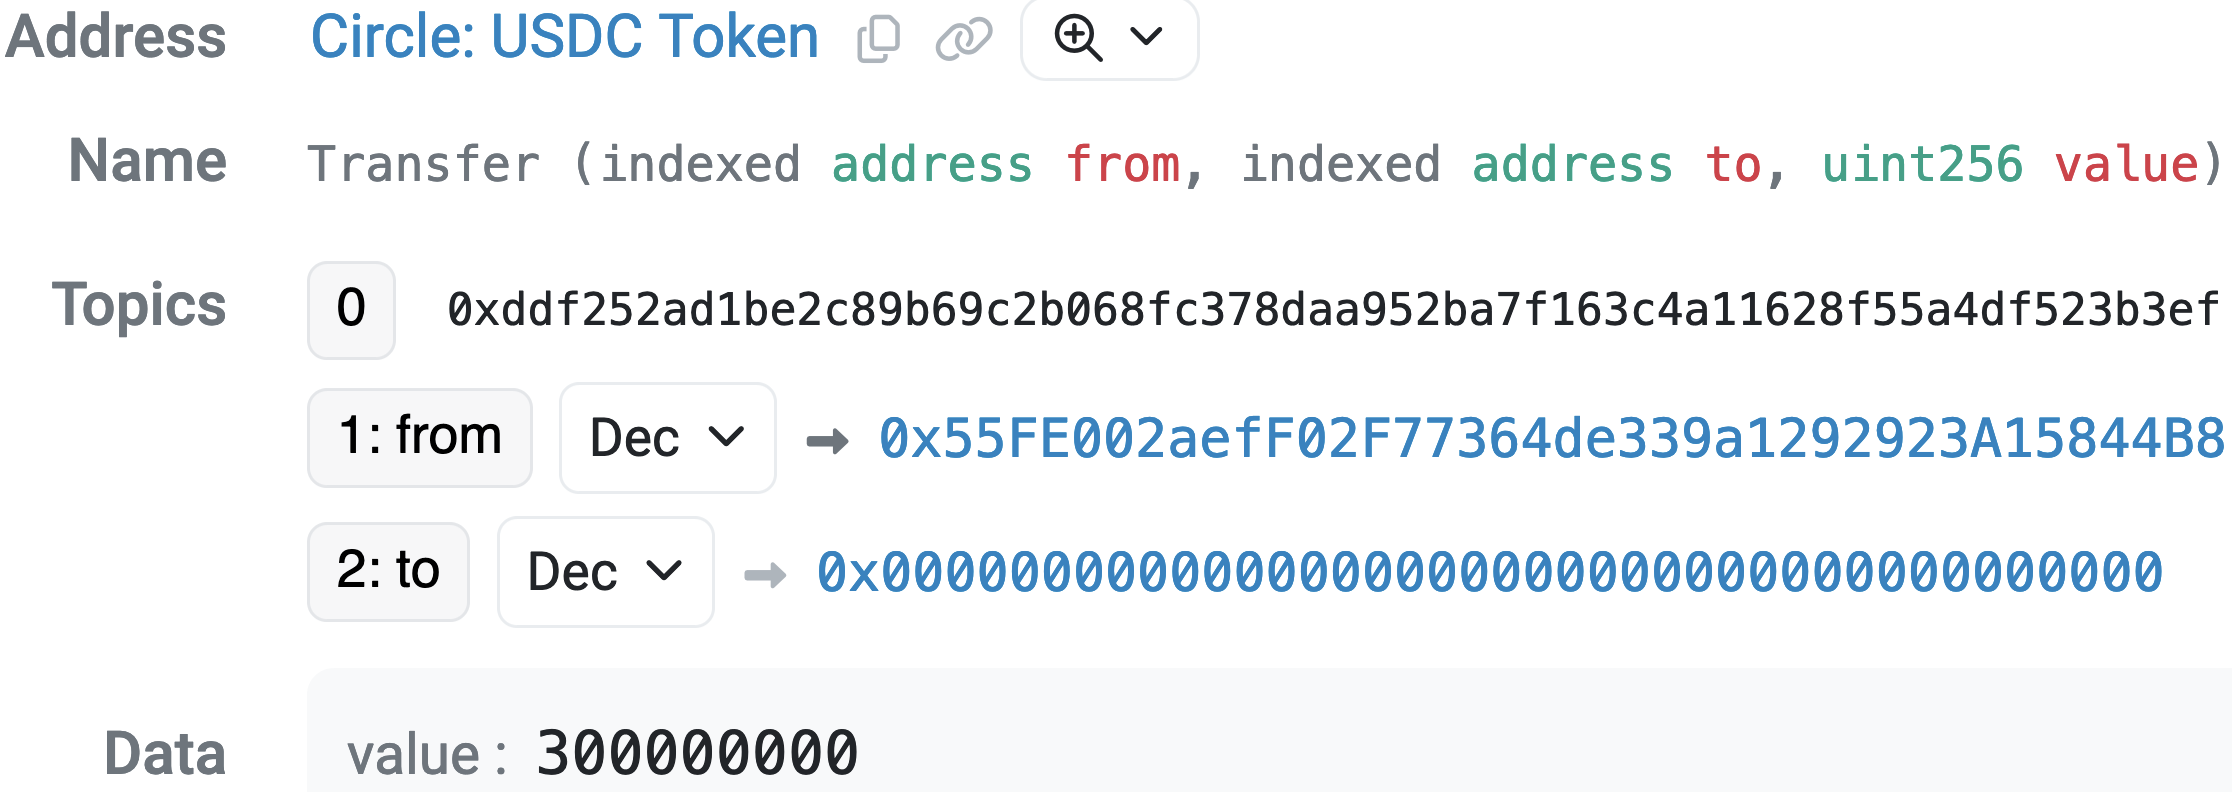
\includegraphics[width=0.7\columnwidth]{fig/token.png}
\caption{Event Emitted by an ERC-20 Token (USDC).}
\label{fig:erc20-event}
\end{figure}

As Figure~\ref{fig:cross-chain} shows, a typical cross-chain token transfer,
i.e., a bridge transaction, consists three phases:

\textbf{1. Deposit (on source chain).}
To initiate a cross-chain token transfer, the user first calls the bridge's
contract on the source chain:
\begin{lstlisting}
deposit(address token, uint256 val, address to) {
  address from = msg.sender;  // user
  address to = address(this); // bridge contract
  // ... validate the ERC-20 token contract
  token.safeTransferFrom(from, to, val);
  emit Deposited(id++, token, from, to, val);
}
\end{lstlisting}
This contract function---a simplified version of the Qubit bridge deposit
function---processes the user's deposit (step 2) by validating the transfer request,
e.g., against a list supported tokens, and then transferring the user's ERC-20
tokens to the bridge contract---recall contracts are accounts with balances.
Then, the function emits an event (step 3) recording the user's deposit details
(including the deposit ID, the ERC-20 token contract address, the recipient on
the destination chain, and value).

\textbf{2. Off-chain relay.}
The emitted event is observed by an off-chain relayer in (step 4),
which constantly monitors the source blockchain.  The relayer first
verifies the authenticity of the deposit event.  If the event is
authentic, the relayer then produces a signed \emph{receipt}
endorsing the deposit (step 5) and, typically, stores the receipt off-chain (step
6).  Finally, this signed receipt is sent to the bridge's withdrawal contract
on the destination blockchain (step 7). Who submits the receipt varies across
bridges---some bridges submit the receipt on the user's behalf (in these cases, the
signed receipt is simply a signed contract-call transaction), while others give
users (and anyone willing to pay gas) the signed receipt and they, in turn,
submit the receipt to the withdrawal contract to complete the transfer. 

\textbf{3. Withdraw (on destination chain).}
The withdrawal contract on the destination chain first processes the withdraw
request by verifying the receipt and transferring the tokens to the recipient
(step 8). In (the simplified) Chainswap's withdraw case, for example, users call:
\begin{lstlisting}
withdraw(uint256 id, address token, address to, 
  uint256 val, Signature[] sigs) {
    _chargeFee();
    // verify receipt
    require(received[id][to] == 0, 'withdrawn');
    for(uint i=0; i < sigs.length; i++) {
      verify_receipt(sigs[i], id, token, to, val);
    }
    received[id][to] = val; // mark as withdrawn
    token.safeTransferFrom(address(this), to, val);
    emit Withdraw(id, token, to, val);
}
\end{lstlisting}
This contract function first charges the caller a fee, then verifies the
deposit details against receipt---both that the deposit was not already
withdrawn and that the receipt signatures are valid---and finally transfers the
tokens to the intended recipient.  I consider a cross-chain transaction
complete when the asset is released to the recipient (step~9).

I expect every cross-chain bridge transaction to uphold the balance invariant:
the value (and kind) of the tokens withdrawn---the outflow---should equal the
value (and kind) of the tokens deposited---the inflow---minus the charged fees.
In practice, they do not.



% \subsection{Cross-Chain Bridges}
% In this section, I begin by providing an example of how a typical cross-chain transaction works. We then discuss the different variants of cross-chain bridges. 
% \subsubsection{A Typical Cross-Chain Transaction}
% Figure~\ref{fig:cross-chain} depicts a typical cross-chain transaction. Starting with the source blockchain, the sender (represented by their EOA) initiates a transaction to transfer assets to the bridge's deposit contract (step 1). The bridge contract then verifies that it has received the assets (step 2). Upon verification, the bridge contract emits an event to record the transfer (step 3). This event is observed by the relaying component (step 4), which typically resides outside and constantly monitors the source blockchain. The relaying component then verifies the authenticity of the event (step 5). If the event is authentic, the relaying component signs the message and stores the signature in a queryable database (step 6). A submitter on the destination blockchain then fetches the signed message from the database (step 7) and sends it to the bridge's withdrawal contract on the destination blockchain (step 8). The bridge contract then verifies the signature (step 9) and transfers the assets to the recipient (step 10). A cross-chain transaction is considered complete when the asset is released to the recipient (step 11).

% % Important things I need in this figure:
%     % source and dst amount
%     % how different vulnerabilities manifest
%         % source
%             % transfer in
%             % verify * emit
%         % relaying component
%             % observe
%             % signs
%         % dst
%             % retrieve & send
%             % verify
%             % transfer out
%     % Players
%         % Sender (in source)
%         % Relayer (in dst)
%         % Receiver (in dst)
    
    



% \subsubsection{Variants of Bridge Implementation}
% Beyond the typical cross-chain transaction described above, there are different ways to implement a cross-chain bridge. We discuss the following variants:

% \textbf{Asset Management.} There are two common ways funds can be released in step 10. The first model is the liquidity pool, which is commonly used when an asset already exists on both blockchains (e.g., USDC already exists on Ethereum and Polygon). Bridges start by creating liquidity pools, to which users can deposit assets and earn fees. When a withdrawal request is made, the bridge releases the funds from the liquidity pool as long as there is sufficient capital in the pool. The second model is mint-and-burn, which can be used regardless of whether the asset exists on the destination blockchain. In this model, the bridge contract mints new tokens on the destination blockchain, which act as representations of the assets on the source blockchain. When a withdrawal request is made, the bridge simply mints new tokens and sends them to the recipient. The recipient can then burn the tokens to receive the original assets on the source blockchain.



% \textbf{Submitter Privilege.} In the flow depicted in Figure~\ref{fig:cross-chain}, once the relaying component has signed the transaction, anyone can fetch the signed message and submit it to the destination blockchain. However, in practice, there is a variant where only privileged EOAs can act as submitters. In this variant, the authenticity of the message is verified by the presence of a privileged key. If bridges choose to operate in this way, they 
% typically simplify step 6 by directly storing the message without signing it.

% \textbf{Transaction Relay.} In the flow depicted in Figure~\ref{fig:cross-chain}, each transaction is relayed individually. In practice, transactions can also be relayed in batches or grouped into a Merkle tree. This approach can improve efficiency. However, while using a Merkle tree is more efficient, it also introduces additional complexity in step 9, where the bridge contract has to verify that a transaction is included in a Merkle tree.

% \textbf{Message Verification Mechanisms.} There are four different mechanisms to verify the authenticity of a message. Namely, external verification, optimistic verification, native verification, and local verification. The details of these mechanisms are not critical for this paper. We provide a brief overview of each model and refer the reader to \alex{cite} for more details. At a high level, external verification indicates that the relaying component resides outside both the source and destination blockchains. The legitimacy of a cross-chain transaction is attested by a third party (or a set of third parties). Native verification, on the other hand, indicates that the relaying component resides within the destination blockchain. In this model, the relaying component typically operates as a light client of the source blockchain and maintains enough information to verify the authenticity of a message from the source blockchain. Optimistic verification improves the efficiency of external verification by assuming that the majority of relayed transactions on the destination blockchain are valid. Instead of attesting to the validity of every transaction, optimistic verification only intervenes when a fraudulent transaction is detected. Finally, local verification means that the two parties involved in a cross-chain transaction (e.g., the sender and the submitter) must cooperate and collaborate for the transaction to succeed.

% \textbf{Token Swap Bridges.} In the above example, tokens released on the destination blockchain are backed by an equivalent amount of assets (less fee) on the source blockchain. However, in practice, bridges can also support token swap. In this case, an asset on the source blockchain is swapped for a different asset on the destination blockchain. For example, a user can swap 1 ETH for 100 USDC. The conversion rate is typically determined by the relaying component and may not be publicly disclosed. 

% \subsubsection{Variants of Verification Mechanism.}
% \textbf{External Verification.} In the most common case, the verification components resides outside both the source and destination blockchains. This is known as an externally verified bridge. The legitimacy and correctness of a cross-chain transaction is determined by a third-party (or a set of third-parties). Common ways to implement external verification include Multi-party Computation and Threshold Signature Scheme.\alex{cite}

% \textbf{Optimistic Verification.} Optimistic Verification improves on the efficiency of external verification by assuming that the majority of transactions are valid. Instead of attesting to the validity of every transaction, optimistic verification only intervenes when a dispute arises. This is known as an optimistic bridge. Concretely, every message that is passed to the destination blockchain is considered "pending" until the dispute window expires. The system relies on one or more honest watchers to dispute the message if it is incorrect. If no dispute arises, the message is considered valid.

% \textbf{Native Verification}
% Contrary to external verification, where the verification component resides outside the source and destination blockchains, the verification component in a natively verified bridge resides within the destination blockchain. Commonly, this is achieved by implementing a light client of the source blockchain within the destination blockchain, which maintains enough information for verifying the authenticity of a message. The security is guaranteed by the validators of the source chain. 


% \textbf{Local Verification}
% \alex{add citation. this is the most confusing one.}
% The basic idea is that the sender and the submitter
% have to cooperate and collaborate for a cross-chain transaction to succeed. 

\subsection{How Bridges Collapse}
In practice, attackers exploited bugs in all three components---the deposit
contract, the relayer, and the withdraw contract---and stole signing keys
to siphon hundreds of thousands of dollars.
%
Figure~\ref{fig:cross-chain} highlights the precise steps in the cross-chain
token transfer that attackers have historically exploited, including:
\begin{CompactItemize}
\item \textbf{Bugs in the deposit contract.} In step 2, the bridge contract
verifies that it has received the correct amount of assets before emitting an
event. Bugs in this verification logic could allow an attacker to deposit a
smaller amount of assets than what is recorded by the bridge in the event (step
3). For example, Qubit's \texttt{deposit} function  (see above) did not properly validate the token address. This bug allowed an attacker to pass \texttt{0} for the token address, so the contract function did not actually transfer any funds from the attacker's account but still emitted a \texttt{Deposit} event which allowed the attacker to withdraw actual tokens on the destination chain~\cite{qubit:rekt}.

\item \textbf{Bugs in the off-chain deposit verification.} In step 5, the
relayer verifies the authenticity of the deposit event emitted by the
bridge contract, including whether the event is emitted by the bridge's
designated contract.  Bridges that do not correctly verify
deposits would allow attackers to withdraw assets that are never deposited.
% ---and this 

\item \textbf{Stolen relayer (or submitter) keys.} In step 5, the relayer signs the deposit receipts which are then submitted to the withdrawal
contract as evidence of a valid deposit. If the relayer key is compromised
(e.g., as with the Ronin bridge~\cite{roninattack}) the attacker can forge a
valid receipt and then withdraw assets that were never deposited by calling
\texttt{withdraw} with the forged receipt.

The same is true for bridges that submit receipts on behalf of users---and
essentially restrict the \texttt{withdraw} callers to privileged submitter
accounts. The bridge submitter keys (step 8) have similarly been compromised
(e.g., as with AnySwap~\cite{anyswapattack}) and used to withdraw
unbacked deposits.

\item \textbf{Bugs in the withdraw verification.} In step 8, the bridge contract
verifies that the messages are signed by the relayer and have not
been replayed. Bugs in this verification logic (e.g., as seen with
Wormhole~\cite{wormholeattack}) have allowed attackers to supply ``valid''
payloads that were not signed by the relayer and replay withdrawal
requests with valid deposit receipts that have already been withdrawn.
\end{CompactItemize}


% Liquidity Pool vs Mint-and-Burn. Example USDC on ETH and Polygon
% Verification Modes
% \subsection{Threat Model}
% In this section, I describe the attack surfaces that are in scope for this paper. Importantly, I assume that deposits and withdrawals are made through designated functions and that funds cannot be withdrawn through functions other than the designated withdrawal function(s). Given this setup, I consider the following attack surfaces:

% \textbf{Buggy Deposit Verification.} In step 2, the bridge contract verifies that it has received the correct amount of assets before emitting an event. Bugs in this verification logic could allow an attacker to deposit a smaller amount of assets than what is recorded by the bridge in the event (step 3).

% \textbf{Buggy Event Verification.} In step 5, the relaying component verifies the authenticity of the event emitted by the bridge contract, including whether the event is emitted by the bridge's designated contract. Failure to do so could allow an attacker to withdraw assets that were never deposited.

% \textbf{Compromised Relaying Key.} In step 6, the relaying component signs the message and stores the signature in a queryable database. If the relaying key is compromised, an attacker could forge a message and withdraw assets that were never deposited.

% \textbf{Compromised Submitter Key.} In step 8, some bridges operate in a privileged submitter mode, where the presence of the privileged submitter key is the only requirement to attest to the authenticity of a message. In this case, if the submitter key is compromised, an attacker could submit a forged message and withdraw assets that were never deposited.

%\textbf{Buggy Withdraw Verification.} In step 9, the bridge contract verifies that the messages are signed by the relaying component and have not been replayed. Bugs in this verification logic could allow an attacker to verify payloads that are not signed by the relaying component or to replay a message that has already been processed.

In this chapter, I assume an attacker can exploit any of the aforementioned
components or otherwise control the relayer (or submitter) keys.
In the next section, I show that this attacker model and our simple
\emph{balance invariant checking} captures the largest attacks on cross-chain
bridges that have happened in the past.  In Sections~\ref{sec:live-audit} I show
that monitoring withdrawals and deposits on the source and destination chains
can be used to detect similar attacks in the future.  Finally, in
Section~\ref{sec:active-protect} I describe an \emph{announce-then-execute} bridge
design that enforces this invariant to prevent attacks before they happen.

I note that while our threat model captures a wide variety of vulnerabilities,
it is not exhaustive.  As with any detection system, an attack that violates one
of our assumptions (e.g., avoids violating the balance invariant by transferring
funds off-bridge or not having a withdrawal, subverts the transaction data used to validate the invariant,
etc.) might succeed.
I similarly consider other smart contract bugs (beyond bugs in deposit and withdrawal functions) and account key compromises out of scope---and instead focus
on the cross-chain bridging aspects which are relatively less well understood.
As I show later, our model captures the largest attacks on
cross-chain bridges that have happened in the past and systems can use
it to prevent similar attacks in the future.


%% While our approach captures a variety of vulnerabilities, it is by no
%% means exhaustive. For example, a key assumption I make is that
%% withdrawal are done through designated withdraw functions. However, if
%% an adversary is able to compromise the key to account that holds the
%% funds for the bridge, they could simply transfer the funds to another
%% account and then withdraw them without going through the designated
%% withdraw function(s). Similarly, if an adversary is able to withdraw
%% funds by repurposing other functions (e.g., the deposit function), our
%% approach would not detect it. Moreover, if an attack transaction does
%% not involve a withdrawal, our approach would not detect it. Last but
%% not least, if an attack is somehow able to profit without breaking the
%% balance invariant, our approach would not detect it.  However, we
%% believe that our approach is a important first step in using
%% accounting principles to protect bridges from theft and that it can be
%% extended to address these and other vulnerabilities in the future.
